\begin{figure}
    \centering
    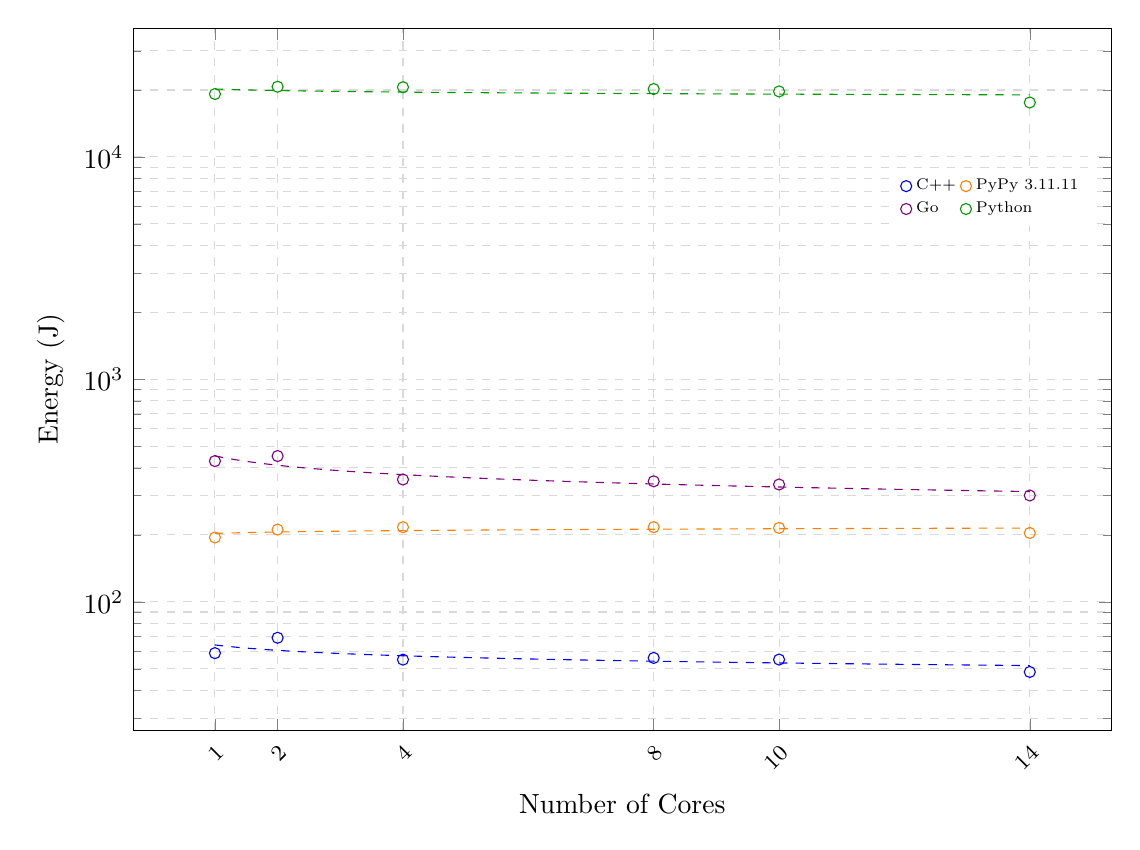
\begin{tikzpicture}
    %% Add a title for the figure
  \begin{semilogyaxis}[
      width=14cm,
      height=10.5cm,
      xlabel={Number of Cores},
      ylabel={Energy (J)},
      ymode=log,
      xmode=linear,
      grid=both,
      minor tick num=1,
      grid style={gray!30,dashed},
      xtick={1,2,4,8,10,14},
      x tick label style={
        font=\footnotesize,
        rotate=45,
        anchor=north east
      },
      legend style={
        at={(0.98,0.8)},
        anchor=north east,
        font=\scriptsize,
        nodes={scale=0.8,transform shape},
        draw=none
      },
      legend columns=2,
      transpose legend,
      legend cell align=left,
    ]
    %% C++ %%
    \addplot[
      blue,
      only marks,
      mark=o,
      mark options={draw=blue,fill=white}
    ]
    table[row sep=\\] {
      x    y      \\
      1    58.79  \\
      2    68.93  \\
      4    54.97  \\
      8    55.94  \\
      10   55.00  \\
      14   48.39  \\
    };
    \addlegendentry{C++}
    % power‐law fit: y = 64.0 * x^(–0.081)
    \addplot[
      blue,
      dashed,
      forget plot,
      domain=1:14,
      samples=200
    ] {64.0 * x^(-0.081)};

    %% Go %%
    \addplot[
      violet,
      only marks,
      mark=o,
      mark options={draw=violet,fill=white}
    ]
    table[row sep=\\] {
      x     y       \\
      1     429.23  \\
      2     452.12  \\
      4     354.64  \\
      8     348.14  \\
      10    336.88  \\
      14    300.66  \\
    };
    \addlegendentry{Go}
    % power‐law fit: y = 453 * x^(–0.140)
    \addplot[
      violet,
      dashed,
      forget plot,
      domain=1:14,
      samples=200
    ] {453 * x^(-0.140)};

    %% PyPy 3.11.11 %%
    \addplot[
      orange,
      only marks,
      mark=o,
      mark options={draw=orange,fill=white}
    ]
    table[row sep=\\] {
      x    y      \\
      1    194.69 \\
      2    211.21 \\
      4    216.53 \\
      8    216.60 \\
      10   214.96 \\
      14   203.92 \\
    };
    \addlegendentry{PyPy 3.11.11}
    % power‐law fit: y = 203 * x^(0.021)
    \addplot[
      orange,
      dashed,
      forget plot,
      domain=1:14,
      samples=200
    ] {203 * x^(0.021)};

    %% Python %%
    \addplot[
      green!60!black,
      only marks,
      mark=o,
      mark options={draw=green!60!black,fill=white}
    ]
    table[row sep=\\] {
      x      y        \\
      1      19183.95 \\
      2      20680.94 \\
      4      20580.73 \\
      8      20198.35 \\
      10     19701.50 \\
      14     17567.03 \\
    };
    \addlegendentry{Python}
    % power‐law fit: y = 20200 * x^(–0.023)
    \addplot[
      green!60!black,
      dashed,
      forget plot,
      domain=1:14,
      samples=200
    ] {20200 * x^(-0.023)};

  \end{semilogyaxis}
\end{tikzpicture}
    \caption{Logarithm Energy consumption of the MBP algorithm in different programming languages.}
    \label{fig:log-mbp-energy}
\end{figure}

\begin{figure}
    \centering
    
    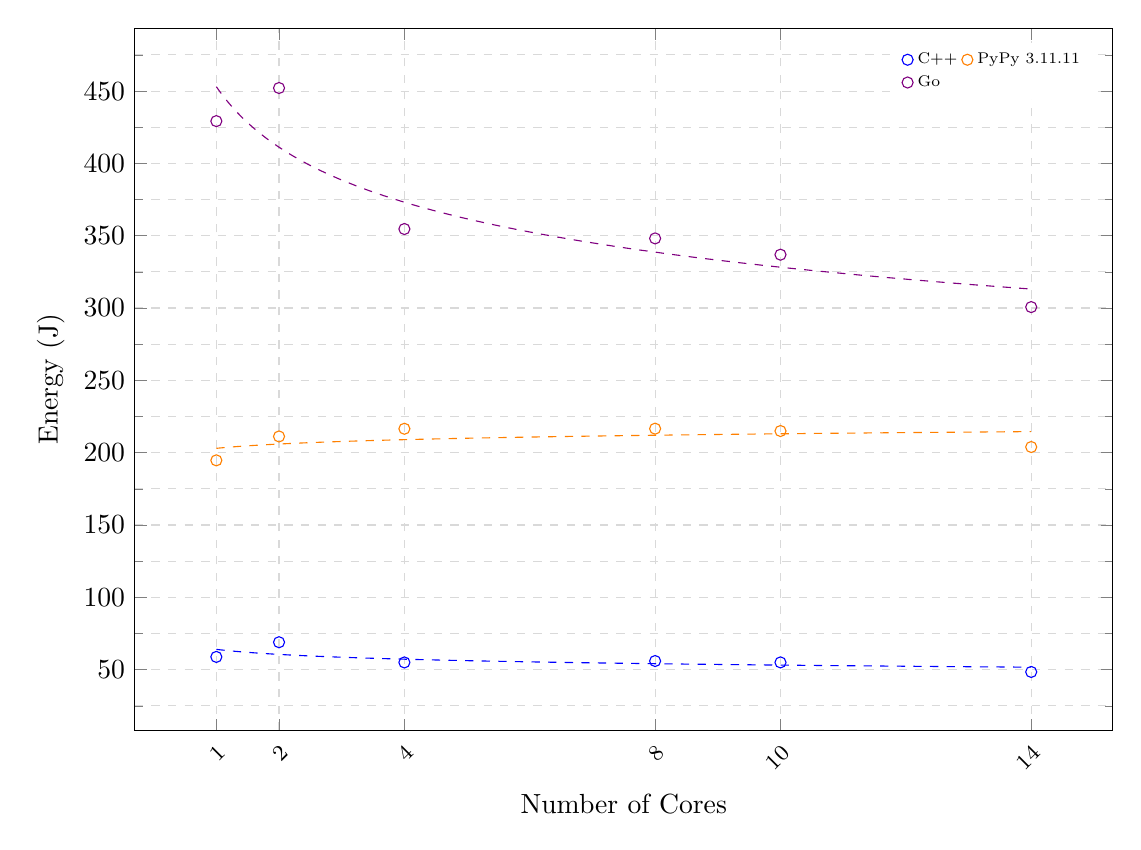
\begin{tikzpicture}
  \begin{axis}[
      width=14cm,
      height=10.5cm,
      xlabel={Number of Cores},
      ylabel={Energy (J)},
      ymode=linear,
      xmode=linear,
      grid=both,
      minor tick num=1,
      grid style={gray!30,dashed},
      xtick={1,2,4,8,10,14},
      x tick label style={
        font=\footnotesize,
        rotate=45,
        anchor=north east
      },
      legend style={
        at={(0.98,0.98)},
        anchor=north east,
        font=\scriptsize,
        nodes={scale=0.8,transform shape},
        draw=none
      },
      legend columns=2,
      transpose legend,
      legend cell align=left,
    ]
    %% C++ %%
    \addplot[
      blue,
      only marks,
      mark=o,
      mark options={draw=blue,fill=white}
    ]
    table[row sep=\\] {
      x    y      \\
      1    58.79  \\
      2    68.93  \\
      4    54.97  \\
      8    55.94  \\
      10   55.00  \\
      14   48.39  \\
    };
    \addlegendentry{C++}
    % power‐law fit: y = 64.0 * x^(–0.081)
    \addplot[
      blue,
      dashed,
      forget plot,
      domain=1:14,
      samples=200
    ] {64.0 * x^(-0.081)};

    %% Go %%
    \addplot[
      violet,
      only marks,
      mark=o,
      mark options={draw=violet,fill=white}
    ]
    table[row sep=\\] {
      x     y       \\
      1     429.23  \\
      2     452.12  \\
      4     354.64  \\
      8     348.14  \\
      10    336.88  \\
      14    300.66  \\
    };
    \addlegendentry{Go}
    % power‐law fit: y = 453 * x^(–0.140)
    \addplot[
      violet,
      dashed,
      forget plot,
      domain=1:14,
      samples=200
    ] {453 * x^(-0.140)};

    %% PyPy 3.11.11 %%
    \addplot[
      orange,
      only marks,
      mark=o,
      mark options={draw=orange,fill=white}
    ]
    table[row sep=\\] {
      x    y      \\
      1    194.69 \\
      2    211.21 \\
      4    216.53 \\
      8    216.60 \\
      10   214.96 \\
      14   203.92 \\
    };
    \addlegendentry{PyPy 3.11.11}
    % power‐law fit: y = 203 * x^(0.021)
    \addplot[
      orange,
      dashed,
      forget plot,
      domain=1:14,
      samples=200
    ] {203 * x^(0.021)};

  \end{axis}
\end{tikzpicture}

    \caption{Linear Energy consumption of the MBP algorithm in different programming languages.}
    \label{fig:linear-mbp-energy}
\end{figure}

\begin{table}
    \centering
    \begin{tabular}{lrrrr}
        \hline
        Cores & C++   & Go     & PyPy 3.11.11 & Python      \\
        \hline
        1     & 58.79  & 429.23  & 194.69       & 19,183.95   \\
        2     & 68.93  & 452.12  & 211.21       & 20,680.94   \\
        4     & 54.97  & 354.64  & 216.53       & 20,580.73   \\
        8     & 55.94  & 348.14  & 216.60       & 20,198.35   \\
        10    & 55.00  & 336.88  & 214.96       & 19,701.50   \\
        14    & 48.39  & 300.66  & 203.92       & 17,567.03   \\
        \hline
    \end{tabular}
    \caption{Power consumption by implementation and core count}
    \label{tab:mbp-power-consumption}
\end{table}